% !TEX root = ../main.tex
\section{Validation, sensitivity and benchmark}
\label{sec:validation}

\subsection{Did high-priority provinces see more cases?}

For each typhoon, the ranking made at the landfall week is compared with the incidence each unit saw over the next four weeks, relative to its own threshold (Table~\ref{tab:valid}, Figure~\ref{fig:valid}). $R$ ranks provinces well for both 2018--2019 storms. $P$ correlates less with cases, as it should: $A$ measures access, not disease. After Ompong, \topTenSurgedOmpong{} of the ten highest-priority provinces surged against a \surgeRateOmpong{} base rate. After Tisoy almost nothing surged (the 2019 season was over), so the top-ten rate is zero and the Brier score is low for the right reason.

\begin{table}[htbp]
\centering
\caption{Backtest per typhoon: units scored, share that surged, Spearman correlation of $R$ and of $P$ with the observed incidence, surge rate among the ten highest-priority units, and the Brier score of $R$.}
\label{tab:valid}
\footnotesize
\begin{tabularx}{\linewidth}{@{}l l r r r r r r L@{}}
\toprule
typhoon & origin & units & surged & $\rho(R, \text{obs})$ & $\rho(P, \text{obs})$ & top-10 surged & Brier $R$ & note \\
\midrule
\tablerows{valid}
\bottomrule
\end{tabularx}
\end{table}

\begin{figure}[htbp]
\centering
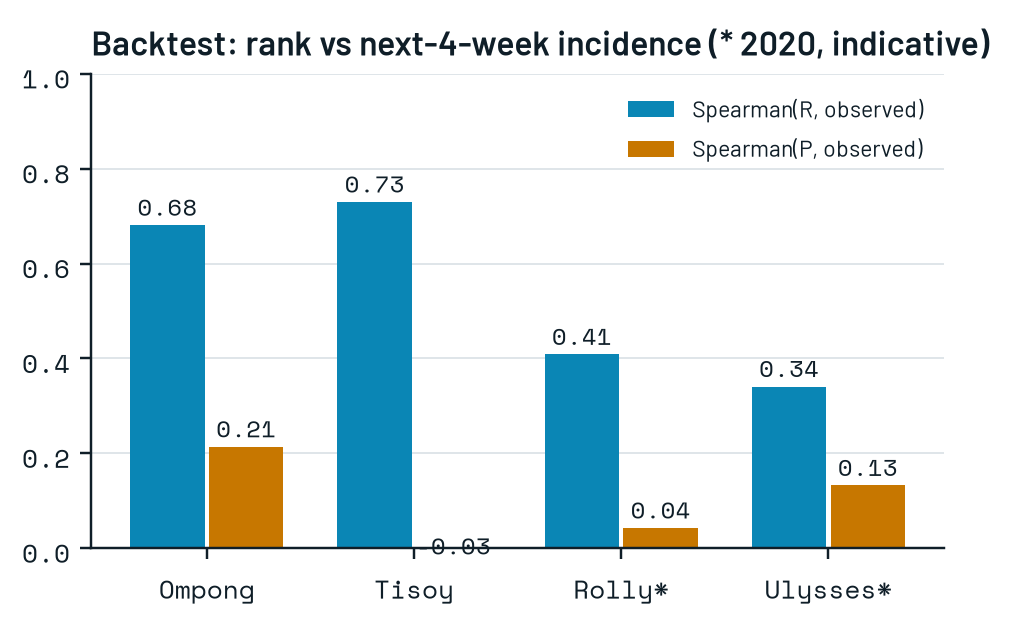
\includegraphics[width=0.62\linewidth]{f10_validation}
\caption{Spearman correlation of each ranking (calibrated $R$) with the observed incidence over the next four weeks, relative to each unit's threshold. Starred storms (2020) are indicative only.}
\label{fig:valid}
\end{figure}

\subsection{Sensitivity}

Table~\ref{tab:sens} gives Kendall's $\tau$ between the base ranking by $P$ (network method) and the ranking under each changed setting. Every variant changes $A$ a little but none reorders the ranking: the spread of $P$ is dominated by $R$. The same variants on the raster method give $\tau \geq \tauMinRaster$. The gale fallback never triggers for these storms.

\begin{table}[htbp]
\centering
\caption{Sensitivity: Kendall's $\tau$ of $P$ against the base settings (network method), and Ompong's mean $A$ under each variant.}
\label{tab:sens}
\footnotesize
\begin{tabular}{@{}l r r r r r@{}}
\toprule
variant & Ompong $\tau$ & Tisoy $\tau$ & Rolly $\tau$ & Ulysses $\tau$ & mean $A$ (Ompong) \\
\midrule
\tablerows{sens}
\bottomrule
\end{tabular}
\end{table}

\subsection{Metro Manila benchmark}

Cutting every road of the National Capital Region (NCR) in NOAH 25-year medium or high hazard leaves \textbf{\benchNCR{}} of NCR without a route within the cut-off rule. A study of the same region reported \litNCRShare{} of people losing access to higher-level care at a 15~cm flood \parencite{tariverdi2023}. The flood and facility definitions differ, so this is an order-of-magnitude check only.
